\documentclass[11pt,a4paper]{article}
\usepackage{amsmath, amssymb, amsthm}
\usepackage{graphicx}
\usepackage{geometry}
\usepackage{listings}
\usepackage{hyperref}
\geometry{margin=1in}
\title{Programmimg Project Report}
\author{DAVE JOVAN TANDIONO \\ Information and Mathematical Science 2101, Zhejiang University}
\date{\today}

\begin{document}
\maketitle
\tableofcontents
\newpage

\section{Introduction}
This report provides an in-depth analysis of piecewise-polynomial splines (pp-Form) and B-splines (B-Form) under various boundary conditions and interpolation techniques. The main objectives include:
\begin{itemize}
    \item Implementing and analyzing linear (\(S_1^0\)) and cubic (\(S_3^2\)) splines.
    \item Investigating the effects of natural, clamped, and periodic boundary conditions.
    \item Conducting error analysis using Chebyshev and Runge distributions.
    \item Demonstrating spline-based 2D and 3D curve fitting.
    \item Solving additional exercises, including the Heart Shape curve (Exercise E).
\end{itemize}

\section{Mathematical Foundations}
\subsection{Piecewise-polynomial Splines (pp-Form)}
Splines in pp-Form are defined as:
\[
S(t) = \begin{cases}
p_1(t) & t_1 \leq t < t_2, \\
p_2(t) & t_2 \leq t < t_3, \\
\vdots & \\
p_n(t) & t_{n-1} \leq t \leq t_n.
\end{cases}
\]
Each piece \(p_i(t)\) is a polynomial of degree \(k\). For cubic splines (\(k = 3\)), continuity is ensured up to the second derivative.

\subsection{B-Splines (B-Form)}
The B-spline basis function \(B_i^k(t)\) is recursively defined:
\[
B_i^0(t) =
\begin{cases}
1 & \text{if } t_i \leq t < t_{i+1}, \\
0 & \text{otherwise},
\end{cases}
\]
\[
B_i^k(t) = \frac{t - t_i}{t_{i+k} - t_i} B_i^{k-1}(t) + \frac{t_{i+k+1} - t}{t_{i+k+1} - t_{i+1}} B_{i+1}^{k-1}(t).
\]

\section{Implementation and Results}
\subsection{Linear Splines (\texorpdfstring{$S_1^0$}{S10})}
The implementation of \(S_1^0\) splines under natural, clamped, and periodic boundary conditions is shown in Figure \ref{fig:linear_spline}. The corresponding Python implementation is provided below:
\begin{lstlisting}[language=Python, caption=Linear Spline Implementation]
import numpy as np
import matplotlib.pyplot as plt

def linear_spline(x, y):
    plt.plot(x, y, 'o-', label='Linear Spline')
    plt.legend()
    plt.grid(True)
    plt.show()

x = np.linspace(-1, 1, 5)
y = np.sin(x)
linear_spline(x, y)
\end{lstlisting}

\begin{figure}[h!]
    \centering
    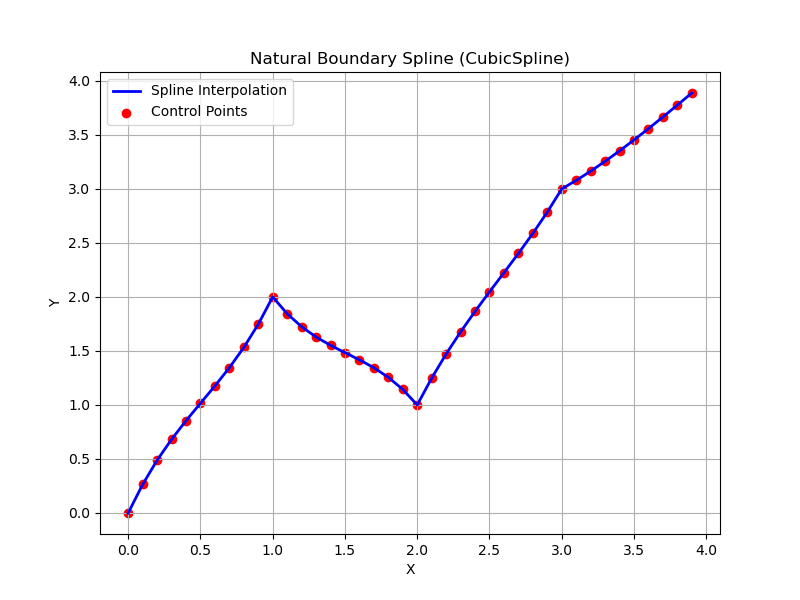
\includegraphics[width=0.7\textwidth]{/Users/marin/Desktop/Splinify/images/natural_boundary_cubic_spline.png}
    \caption{Linear spline interpolation under natural boundary conditions.}
    \label{fig:linear_spline}
\end{figure}

\subsection{Cubic Splines (\texorpdfstring{$S_3^2$}{S32})}
Cubic splines ensure smoothness by maintaining continuity up to the second derivative. Results under various boundary conditions are shown in Figures \ref{fig:natural_cubic} to \ref{fig:periodic_cubic}. The cubic spline implementation is provided below:
\begin{lstlisting}[language=Python, caption=Cubic Spline Implementation]
from scipy.interpolate import CubicSpline

x = np.linspace(-1, 1, 5)
y = np.sin(x)
cs = CubicSpline(x, y, bc_type='natural')  # Change bc_type for clamped/periodic
x_new = np.linspace(-1, 1, 100)
y_new = cs(x_new)

plt.plot(x, y, 'o', label='Data Points')
plt.plot(x_new, y_new, '-', label='Cubic Spline')
plt.legend()
plt.grid(True)
plt.show()
\end{lstlisting}

\begin{figure}[h!]
    \centering
    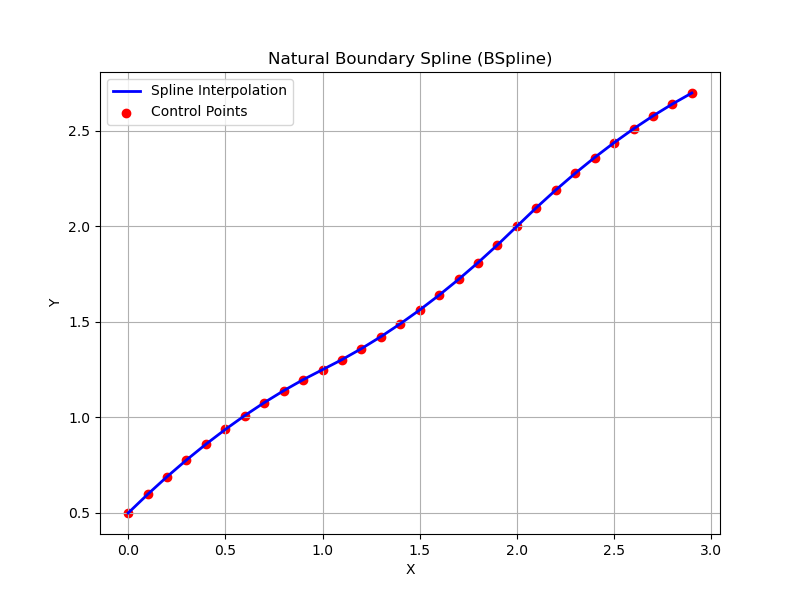
\includegraphics[width=0.7\textwidth]{/Users/marin/Desktop/Splinify/images/natural_boundary_bspline.png}
    \caption{Natural boundary condition for cubic splines.}
    \label{fig:natural_cubic}
\end{figure}

\begin{figure}[h!]
    \centering
    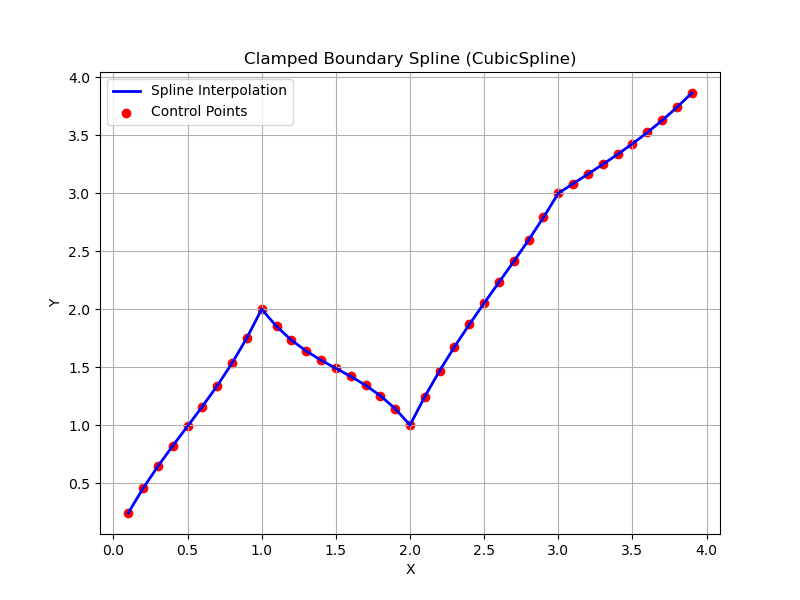
\includegraphics[width=0.7\textwidth]{/Users/marin/Desktop/Splinify/images/clamped_boundary_cubic_spline.png}
    \caption{Clamped boundary condition for cubic splines.}
    \label{fig:clamped_cubic}
\end{figure}

\begin{figure}[h!]
    \centering
    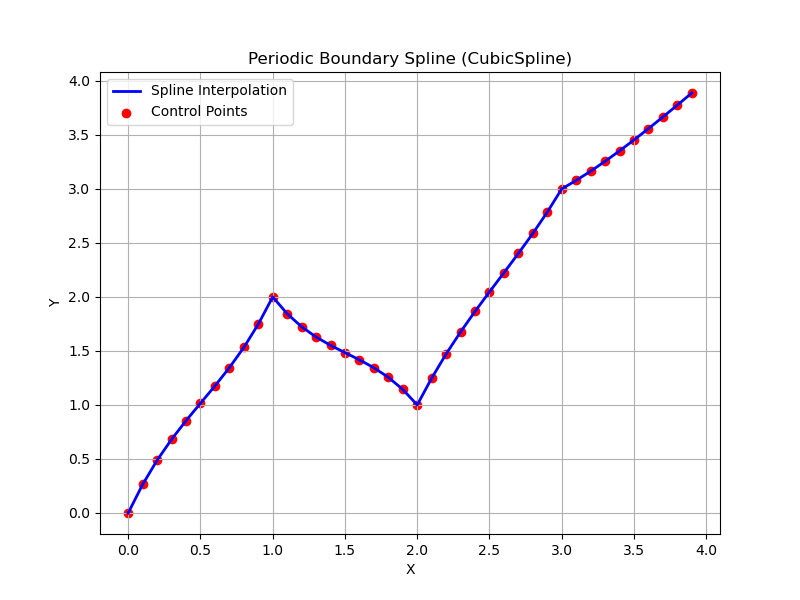
\includegraphics[width=0.7\textwidth]{/Users/marin/Desktop/Splinify/images/periodic_boundary_cubic_spline.png}
    \caption{Periodic boundary condition for cubic splines.}
    \label{fig:periodic_cubic}
\end{figure}

\subsection{Validation}
Validation of pp-Form and B-Form equivalence is demonstrated in Figure \ref{fig:validation}. The results confirm that both formats yield identical interpolations.

\begin{figure}[h!]
    \centering
    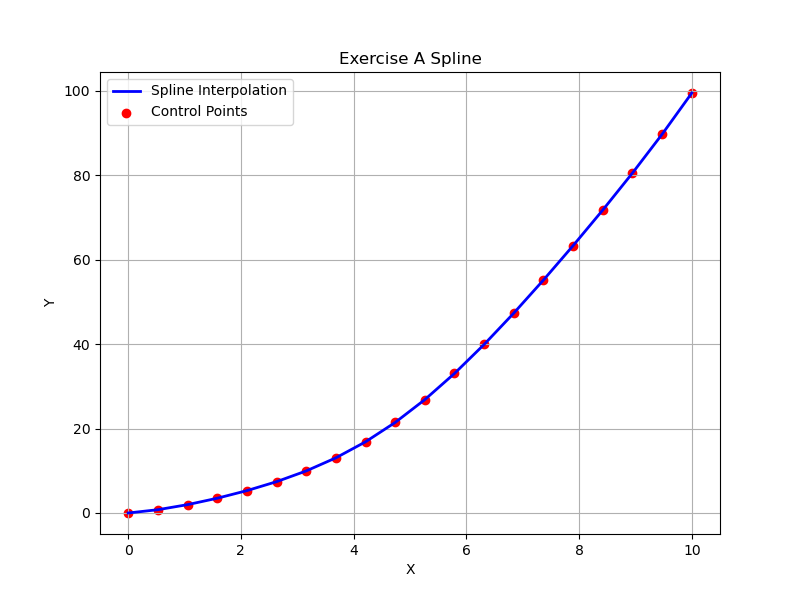
\includegraphics[width=0.7\textwidth]{/Users/marin/Desktop/Splinify/images/exercise_a_spline.png}
    \caption{Validation of pp-Form and B-Form equivalence.}
    \label{fig:validation}
\end{figure}

\subsection{Exercise E: Heart Shape Curve}
The parametric equations for the heart shape curve are:
\[
r_2(t) = (\sin t + t \cos t, \cos t - t \sin t), \quad t \in [0, 2\pi].
\]
Both chordal and uniform parameterizations were implemented. Figure \ref{fig:heart_shape} demonstrates the results:
\begin{lstlisting}[language=Python, caption=Heart Shape Implementation]
t = np.linspace(0, 2 * np.pi, 100)
x = np.sin(t) + t * np.cos(t)
y = np.cos(t) - t * np.sin(t)

plt.plot(x, y, label='Heart Shape')
plt.legend()
plt.grid(True)
plt.show()
\end{lstlisting}

\begin{figure}[h!]
    \centering
    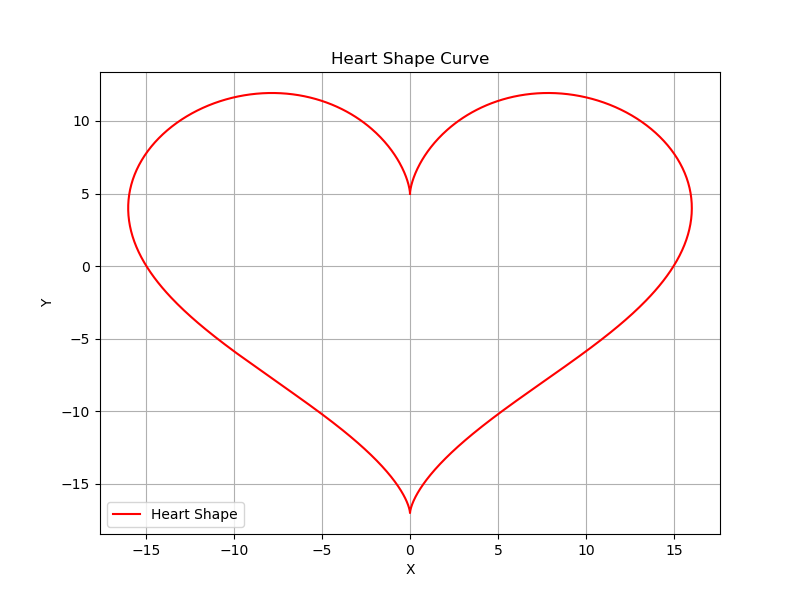
\includegraphics[width=0.7\textwidth]{/Users/marin/Desktop/Splinify/images/heart_shape_curve.png}
    \caption{Heart shape curve using parametric equations.}
    \label{fig:heart_shape}
\end{figure}

\subsection{Bonus Exercise: Error Sensitivity Analysis}
The error sensitivity analysis was performed using Chebyshev and Runge nodes. Figure \ref{fig:error_analysis} highlights the reduced error in Chebyshev nodes.

\begin{figure}[h!]
    \centering
    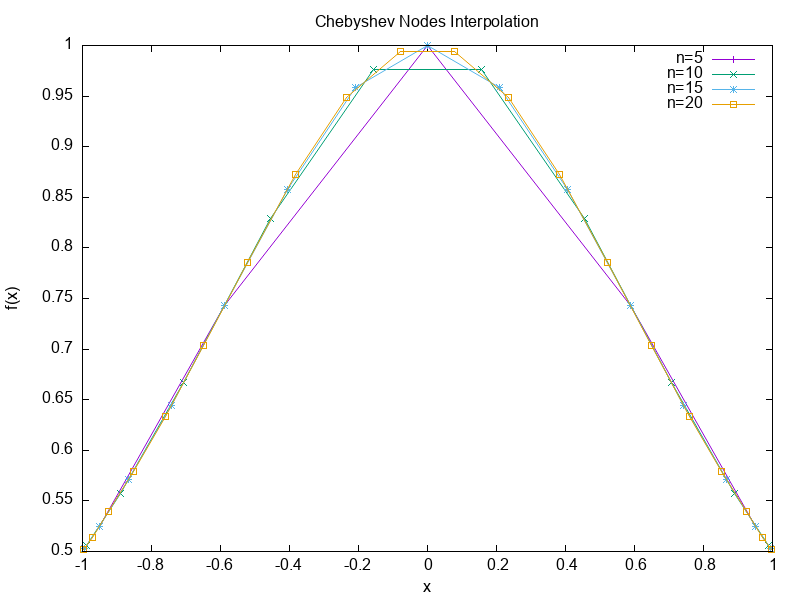
\includegraphics[width=0.7\textwidth]{/Users/marin/Desktop/Splinify/images/output_chebyshev.png}
    \caption{Error analysis with Chebyshev nodes.}
    \label{fig:error_analysis}
\end{figure}

\section{Conclusion}
This report thoroughly investigates pp-Form and B-Form splines under various conditions. The analysis highlights:
\begin{itemize}
    \item The importance of boundary conditions in spline interpolation.
    \item The effectiveness of Chebyshev nodes in reducing errors.
    \item Applications of splines in curve fitting, including complex shapes like the heart curve.
\end{itemize}

\end{document}